\section{Inserção}

\begin{frame}[fragile]{Inserção em árvores binárias de busca}
    \begin{itemize}
	    \item O algoritmo a seguir insere um elemento $x$ em uma árvore binária de busca:

	\begin{enumerate}
		\item Começe no nó raiz

		\item Enquanto o nó a ser avaliado for não-nulo:

		\begin{enumerate}[i.]
            \item seja $y$ a informação armazenada no nó a ser avaliado

            \item se $x$ for menor do que $y$, vá para a raiz da subárvore da esquerda

            \item caso contrário, vá para a raiz da subárvore da direita
		\end{enumerate}

		\item Insira um novo nó com a informação igual ao valor a ser inserido como { filho} do último nó não-nulo, na posição adequada
	\end{enumerate}

        \item No pior caso, o algoritmo visita todos os $N$ nós da árvore, de modo que este algoritmo tem complexidade $O(N)$

    \end{itemize}
\end{frame} 

\begin{frame}[fragile]{Exemplo de inserção em árvore binária de busca}

    \begin{tikzpicture}

        \begin{scope}{shift={(3,1)}}
            \node (X) at (1, 6) { Elemento a ser inserido: \textcolor{blue}{14}};

            \node[circle,draw] (D) at (6, 5) { $25$ };
            \node[circle,draw] (C) at (4, 3) { $9$ };
            \node[circle,draw] (E) at (8, 3) { $63$ };
            \node[circle,draw] (F) at (7, 1) { $47$ };
            \node[circle,draw] (A) at (3, 1) { $1$ };
            \node[circle,draw] (B) at (5, 1) { $23$ };
            \node[circle,draw] (G) at (9, 1) { $80$ };
            \node[opacity=0,circle,draw] (H) at (4, -1) { $14$ };

            \draw (A) -- (C);
            \draw (B) -- (C);
            \draw (C) -- (D);
            \draw (D) -- (E);
            \draw (E) -- (F);
            \draw (E) -- (G);
            \draw[opacity=0] (B) -- (H);

        \end{scope}
    \end{tikzpicture}

\end{frame}

\begin{frame}[fragile]{Exemplo de inserção em árvore binária de busca}

    \begin{tikzpicture}

        \begin{scope}{shift={(3,1)}}
            \node (X) at (1, 6) { Elemento a ser inserido: \textcolor{blue}{14}};

            \node[circle,draw,fill=green!30] (D) at (6, 5) { $25$ };
            \node[circle,draw] (C) at (4, 3) { $9$ };
            \node[circle,draw] (E) at (8, 3) { $63$ };
            \node[circle,draw] (F) at (7, 1) { $47$ };
            \node[circle,draw] (A) at (3, 1) { $1$ };
            \node[circle,draw] (B) at (5, 1) { $23$ };
            \node[circle,draw] (G) at (9, 1) { $80$ };
            \node[opacity=0,circle,draw] (H) at (4, -1) { $14$ };

            \draw (A) -- (C);
            \draw (B) -- (C);
            \draw (C) -- (D);
            \draw (D) -- (E);
            \draw (E) -- (F);
            \draw (E) -- (G);
            \draw[opacity=0] (B) -- (H);

        \end{scope}
    \end{tikzpicture}

\end{frame}

\begin{frame}[fragile]{Exemplo de inserção em árvore binária de busca}

    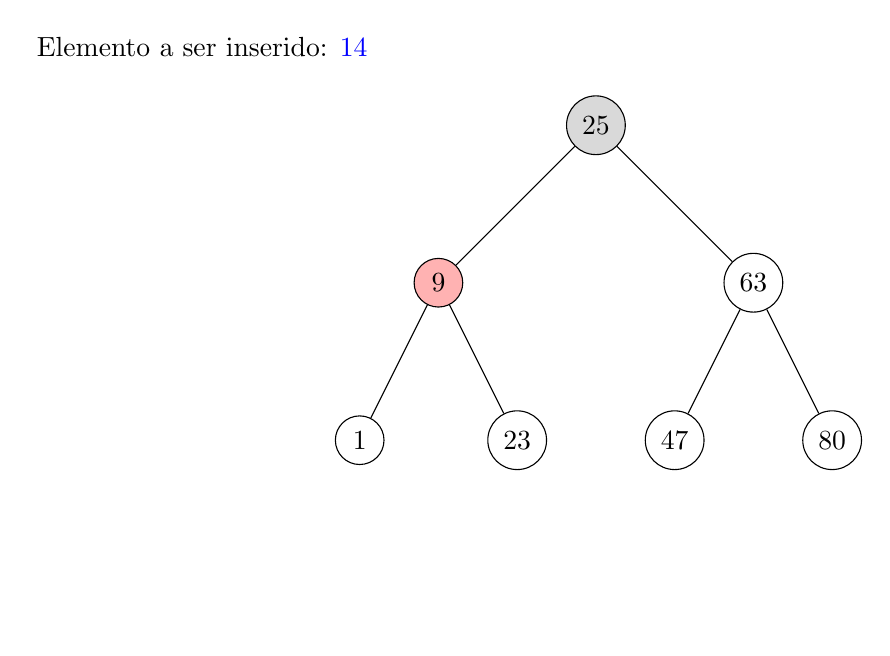
\begin{tikzpicture}

        \begin{scope}{shift={(3,1)}}
            \node (X) at (1, 6) { Elemento a ser inserido: \textcolor{blue}{14}};

            \node[circle,draw,fill=gray!30] (D) at (6, 5) { $25$ };
            \node[circle,draw,fill=red!30] (C) at (4, 3) { $9$ };
            \node[circle,draw] (E) at (8, 3) { $63$ };
            \node[circle,draw] (F) at (7, 1) { $47$ };
            \node[circle,draw] (A) at (3, 1) { $1$ };
            \node[circle,draw] (B) at (5, 1) { $23$ };
            \node[circle,draw] (G) at (9, 1) { $80$ };
            \node[opacity=0,circle,draw] (H) at (4, -1) { $14$ };

            \draw (A) -- (C);
            \draw (B) -- (C);
            \draw (C) -- (D);
            \draw (D) -- (E);
            \draw (E) -- (F);
            \draw (E) -- (G);
            \draw[opacity=0] (B) -- (H);

        \end{scope}
    \end{tikzpicture}

\end{frame}

\begin{frame}[fragile]{Exemplo de inserção em árvore binária de busca}

    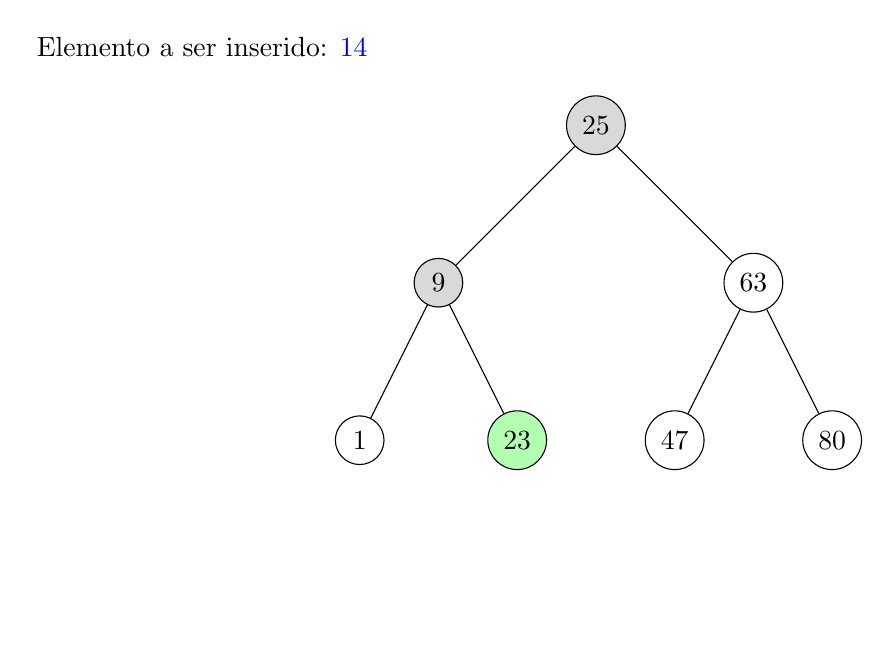
\begin{tikzpicture}

        \begin{scope}{shift={(3,1)}}
            \node (X) at (1, 6) { Elemento a ser inserido: \textcolor{blue}{14}};

            \node[circle,draw,fill=gray!30] (D) at (6, 5) { $25$ };
            \node[circle,draw,fill=gray!30] (C) at (4, 3) { $9$ };
            \node[circle,draw] (E) at (8, 3) { $63$ };
            \node[circle,draw] (F) at (7, 1) { $47$ };
            \node[circle,draw] (A) at (3, 1) { $1$ };
            \node[circle,draw,fill=green!30] (B) at (5, 1) { $23$ };
            \node[circle,draw] (G) at (9, 1) { $80$ };
            \node[opacity=0,circle,draw] (H) at (4, -1) { $14$ };

            \draw (A) -- (C);
            \draw (B) -- (C);
            \draw (C) -- (D);
            \draw (D) -- (E);
            \draw (E) -- (F);
            \draw (E) -- (G);
            \draw[opacity=0] (B) -- (H);

        \end{scope}
    \end{tikzpicture}

\end{frame}

\begin{frame}[fragile]{Exemplo de inserção em árvore binária de busca}

    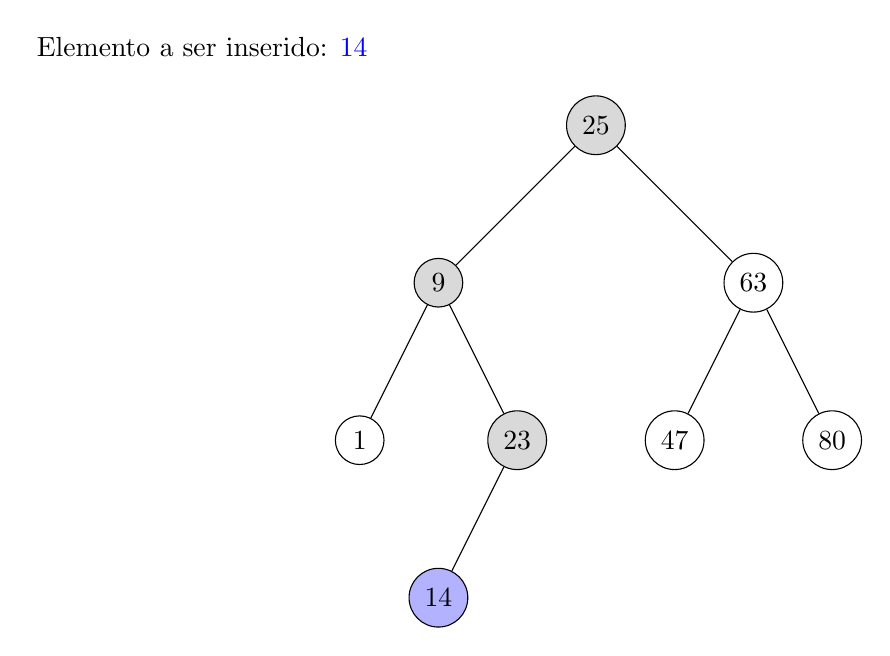
\begin{tikzpicture}

        \begin{scope}{shift={(3,1)}}
            \node (X) at (1, 6) { Elemento a ser inserido: \textcolor{blue}{14}};

            \node[circle,draw,fill=gray!30] (D) at (6, 5) { $25$ };
            \node[circle,draw,fill=gray!30] (C) at (4, 3) { $9$ };
            \node[circle,draw] (E) at (8, 3) { $63$ };
            \node[circle,draw] (F) at (7, 1) { $47$ };
            \node[circle,draw] (A) at (3, 1) { $1$ };
            \node[circle,draw,fill=gray!30] (B) at (5, 1) { $23$ };
            \node[circle,draw] (G) at (9, 1) { $80$ };
            \node[circle,draw,fill=blue!30] (H) at (4, -1) { $14$ };

            \draw (A) -- (C);
            \draw (B) -- (C);
            \draw (C) -- (D);
            \draw (D) -- (E);
            \draw (E) -- (F);
            \draw (E) -- (G);
            \draw (B) -- (H);

        \end{scope}
    \end{tikzpicture}

\end{frame}

\begin{frame}[fragile]{Implementação da inserção em uma BST}
    \inputsnippet{cpp}{1}{20}{codes/insert.cpp}
\end{frame}

\begin{frame}[fragile]{Implementação da inserção em uma BST}
    \inputsnippet{cpp}{22}{42}{codes/insert.cpp}
\end{frame}

\begin{frame}[fragile]{Notas sobre a inserção}

	\begin{itemize}
		\item A inserção { não} modifica a estrutura da árvore, { exceto} no que se refere a acomodação do novo elemento.

        \item Deste modo, a propriedade da árvore binária de busca (BST) fica preservada  

		\item O algoritmo que localiza o nó onde ocorrerá a inserção é semelhante ao código 
            utilizado para buscar elementos na árvore

		\item A inserção pode desbalancear a árvore, isto é, pode fazer com que, em um determinado 
            nó, uma das 
            subárvores tenha um número de nós significativamente maior do que a outra

        \item A inserção de um série de elementos em ordem crescente ou decrescente leva a 
            uma árvore desbalanceada degenerada, que tem mesma estrutura de uma lista encadeada

        \item Esta árvore degenerada configura o pior caso do algoritmo
	\end{itemize}

\end{frame}
